\chapter{ STATE OF THE ART}

This chapter reviews the most relevant developments across four intersecting areas that inform the design of intelligent systems for urban crime analysis: (1) large language models for urban reasoning, (2) LLMs applied to code generation and data analysis, (3) publicly available crime datasets, and (4) visual analytics tools for crime exploration. These domains form the technological and methodological basis for this research.

% We highlight how recent progress in LLM capabilities—such as spatial reasoning, instruction following, and multimodal integration—has enabled new forms of interactive analysis for complex urban phenomena. At the same time, the growing availability of open crime datasets and advances in geospatial visualization tools have paved the way for more accessible and interpretable crime intelligence platforms.


\section{Large-Language Models for Urban Scenarios}

Recent advances show that LLMs are increasingly being adapted to address urban computing tasks. Recent methods show that these models can handle both regression tasks, such as forecasting, and more complex applications, such as participating in agentic workflows to address user queries about urban phenomena.

\citet{Li2024UrbanGPT} proposes UrbanGPT, a spatio-temporal LLM for forecasting urban dynamics such as traffic flows and crime rates. The model receives spatial and time series information through the prompt, then employs a spatio-temporal dependency encoder and a lightweight alignment module to project these representations into the LLM's latent space, achieving performance on par with or surpassing state-of-the-art models in multiple datasets. 

Complementing this, \cite{Jiang2024UrbanLLM} leverage the agentic capabilities of LLMs to decompose urban-related queries into structured sub-tasks (e.g., forecasting, anomaly detection, POI recommendation, etc). This approach, termed UrbanLLM, assigns each sub-task to a specialised model from a curated model zoo, and integrates the results into a unified response.

Recent research from Google has explored the use of foundation models for geospatial reasoning \citep{2025GoogleGeospatialReasoning}. It introduces an agentic workflow powered by Gemini to assist users in tasks such as visualizing pre and post disaster scenarios or conducting damage assessments. Their approach integrates diverse modalities: maps, weather data, and satellite imagery, and highlights the need for foundation models capable of aligning heterogeneous spatial information (Figure \ref{fig:geospatial_reasoning}). Alongside UrbanGPT's forecasting capabilities and UrbanLLM's model orchestration, this work exemplifies the broader movement toward multimodal LLM-based systems designed to address complex urban challenges at scale.

Another study from Google introduces Visual Chronicles \citep{Deng2025VisualChronicles}, a multimodal LLM-based system designed to identify and describe frequently occurring visual changes across urban environments using a dataset provided by Google Street View imagery. It leverages a vast collection of geolocated, timestamped images to identify trends without requiring labeled training data. To overcome the limitations of MLLMs in processing such massive datasets, the authors design a scalable pipeline that enables efficient retrieval, comparison, and semantic analysis of visual patterns across both space and time.

\begin{figure}[hbtp]
  \centering
  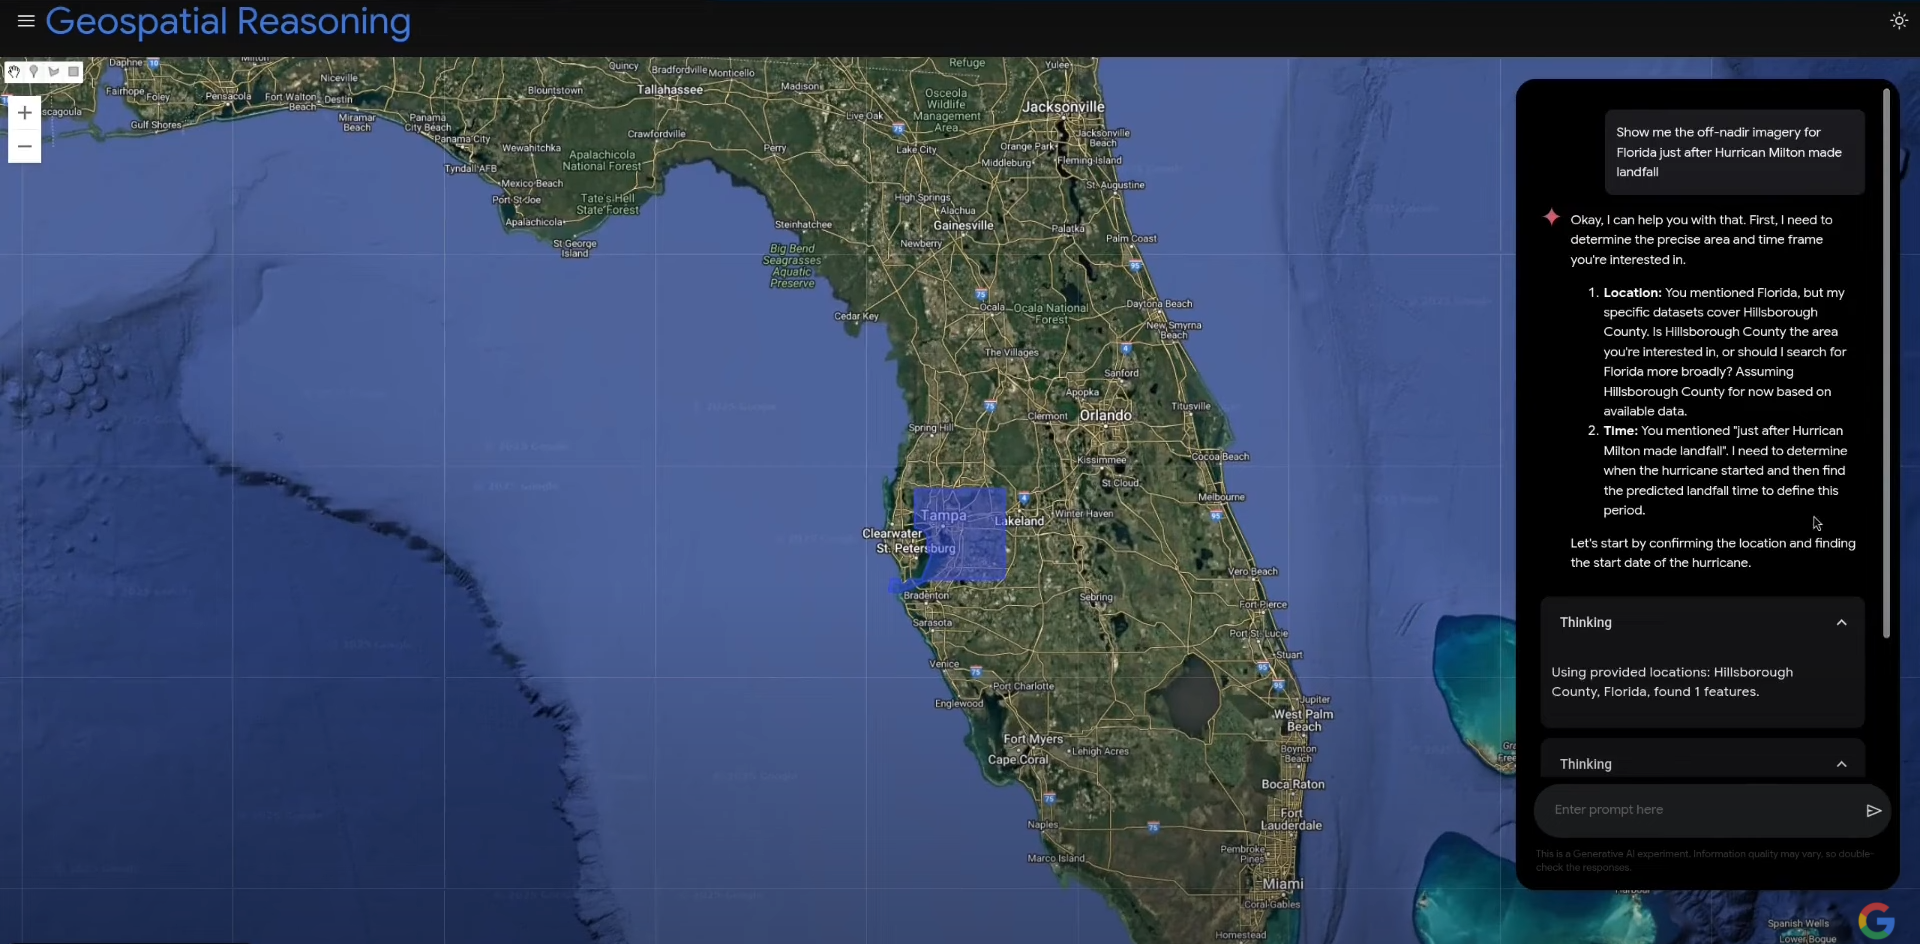
\includegraphics[width=0.95\textwidth]{images/geospatial_reasoning.png}
  \caption{Geospatial Reasoning by Google Research: Demo of chat application powered by Gemini, capable of answering questions about urban phenomena using maps, weather data, and satellite imagery.}
  \label{fig:geospatial_reasoning}
\end{figure}


% \citep{Deng2025VisualChronicles} highlight the system's ability to uncover temporal patterns using MLLMs, capitalizing on their open-ended semantic understanding capabilities. Given that the datasets are several orders of magnitude too large for an MLLM to process as context, the system employs innovative techniques to manage and analyze the data effectively.

% There are more LLMs on Urban Applications: See UrbanLLM paper
% \citep{Zhang2023GeoGPT}



\section{Large-Language Models for Coding-Tasks}

Large language models such as Llama 3 \citep{Grattafiori2024Llama3} already display substantial, general-purpose coding, instruction-following and reasoning skills. In addition, a wave of code-specialised models e.g., Seed-Coder, OpenCodeReasoning, Qwen 2.5-Coder, NuminaMath-7B-TIR, and Code Llama pushes state-of-the-art accuracy on competitive-programming, software-engineering benchmarks, and mathematical problem solving using Python code \citep{Seed2025SeedCoder, Ahmad2025OCRNVidia, Hui2024Qwen25Coder, Roziere2024CodeLlama, Moshkov2025AIMO2, Yin2024MuMathCode, Gou2024ToRA}. These models are constantly improved and frequently surpassed by even newer architectures, reflecting the rapid pace of progress in this area.

Despite the rapid progress in LLMs for code generation, the availability of standardized benchmarks specifically tailored to data science tasks remains limited. Only a handful of recent datasets address this gap: for example, DS‑1000 \citep{Lai2022DS1000} defines 1,000 realistic Python data-analysis problems (with Pandas, NumPy, etc.) collected from StackOverflow, and DataSciBench \citep{Zhang2025DataSciBench} is a recently published comprehensive LLM benchmark covering diverse data-science tasks with an innovative framework of evaluation.

In contrast, the text-to-SQL domain (closely related to data analysis) has more established benchmarks and model work. For example, \cite{Dominguez2024BlarSQL} demonstrated that fine-tuned Llama2 and Code Llama models can decompose database queries and achieve SQL accuracy comparable to GPT-4 on natural-language-to-SQL tasks. Similarly, Snowflake's Arctic-Text2SQL model \citep{Yao2025ArcticText2SQLR1}, trained with reinforcement learning and comprising 7B parameters, achieves state-of-the-art execution accuracy across six standard NL2SQL benchmarks, and currently holds the top single-model position on the BIRD leaderboard \citep{Li2023BirdSQL}. On the enterprise side, systems like QueryGPT \citep{Uber2024QueryGPT} approach this challenge at scale, using an agent-based multi-step pipeline powered by GPT-4 to reliably generate SQL queries adapted to the structure of their internal relational data models.


Most widely used Text2SQL benchmarks, such as BIRD and Spider, are limited to a single SQL dialect and lack support for geospatial operations, including buffer queries and interactions with polygon data types \citep{Li2023BirdSQL, Yu2019Spider}. To address these limitations, this thesis adopts a different approach: instead of relying on SQL, the LLM is used to generate Python code that primarily utilizes the `pandas` and `geopandas` libraries. This strategy avoids SQL dialect constraints and leverages the LLM's strengths in code generation.

% \section{RAG Techniques for Complex Data}

% % * Introduction
% Retrieval-Augmented Generation (RAG) frameworks aim to enhance LLMs by integrating external sources of knowledge, such as structured databases, time series, or knowledge graphs. Recent research has extended RAG beyond textual documents to support spatial, temporal, and graph-based data retrieval.

% % * Spatial RAG
% \citep{Yu2025SpatialRAG} extends RAG to spatial tasks by integrating sparse spatial retrieval (SQL-based queries) with dense semantic retrieval (LLM-based similarity). Their method introduces three preprocessing steps to help the LLM generate complete and executable SQL queries, addressing its limitations in query formulation.
% % , addressing the common challenge of LLMs struggling to construct such queries directly from user input.

% % * RAG on temporal data
% In the temporal domain, \citep{Yang2024TimeRAG} apply RAG to the context of time series forecasting using Dynamic-Time Warping (DTW) as a distance metric to retrieve similar waveforms and trends, given a time serie as a query. The retrieved information is then utilized to improve the LLM forecasting accuracy. 

% % * RAG on graphs
% Other works, combine RAG techniques and hybrid approaches to address question-answering over textual knowledge graphs. One such example is \citep{He2024GRetriever}, who introduce G-Retriever, a flexible QA framework for knowledge graphs that incorporates a RAG into its pipeline. The framework separates node entities and edge information into two distinct embedding spaces. Using cosine similarity, it retrieves the most relevant nodes and edges for the query and reconstructs the subgraph using the Prize-Collecting Steiner Tree (PCST) algorithm. The final answer is generated by a hybrid GNN-LLM, which processes the retrieved subgraph both as text in the query prompt and through a graph encoder aligned with the LLM's token space.

% Building on this idea of graph-based retrieval, \citep{Hu2024GRAG} map textual subgraphs directly to an embedding space, allowing for the retrieval of relevant subgraphs based on their semantic similarity to the query. Then applied techniques to merging and pruning the retrieved subgraphs to improve the quality of the final answer. 

% Recent work from \citep{Guo2024LightRAG} propose LightRAG, a fully prompt-driven framework that extracts knowledge graphs, generates keywords at multiple granularities, retrieves from both vector and graph indexes, and supports fast incremental updates.

% % TODO: \citep{Edge2025GraphRAG}
% % \citep{Xiao2024TimeRAG}
% % \citep{Chen2025KGRAGSurvey}



\section{Open Crime Datasets}

Among the most popular datasets for crime analysis are the Chicago Crime dataset \citep{ChicagoDataset} and the New York City Crime dataset \citep{NYCDataset}. These datasets contain detailed records of reported crimes, including information on the type of crime, location, time, and other relevant attributes. They have been widely used in various research studies and applications related to crime prediction, analysis, and visualization.

Beyond the United States, similar efforts have been made in Latin America. In Brazil, for example, crime datasets are made publicly available at the state level through open data platforms. These resources have supported a range of research projects, including \citep{Garcia2022CriPAV} and \citep{Waqar2025CrimePredictionGNN}, which process and analyze regional crime patterns or develop predictive models.

More recently, large-scale initiatives have emerged in Asia. \citep{Zhang2025CrimeDatasetChina} introduces a large-scale crime dataset from China, comprising approximately 1 million records. The dataset spans 31 provincial-level administrative regions, 222 city-level divisions, and 548 county-level jurisdictions across mainland China. Unlike the structured records in the aforementioned datasets, this resource was constructed by extracting crime information from unstructured judicial documents using LLMs, enabling broader geographic and semantic coverage. Additionally, it includes detailed fields such as case descriptions, victim and defendant information, and final judgments, offering more possibilities for anlysis and research.



\section{Crime-Data Visualization Tools}

% In the context of crime data analysis, several visualization systems have been proposed to support pattern recognition, hotspot identification, and urban context interpretation. These tools typically integrate geospatial data with interactive visual analytics techniques to assist expert users in understanding complex crime patterns.

A range of visualization systems have been developed to support crime data analysis, each advancing the integration of geospatial analytics and interactive exploration. Early tools such as CrimeVis \citep{Silva2017CrimeVisAI} enabled users to interactively explore crime statistics across 138 police districts in Rio de Janeiro from 2003 to 2015, employing coordinated maps, parallel coordinates, and brushing-and-linking to correlate crime data with socio-economic indicators and evaluate the effects of public-safety policies. 

Expanding upon the previous work, Mirante \citep{Garcia2020MiranteAV} introduced a street-level discretization by aggregating incidents on nodes and edges of the road network, allowing for the identification of micro-scale hotspot seasonality through linked heatmaps, histograms, and temporal evolution views.

Subsequent systems have incorporated advanced analytical techniques to deepen insight into spatio-temporal crime patterns. CrimAnalyzer \citep{Garcia2021CrimAnalyzer} integrates visual analytics with Non-negative Matrix Factorization (NMF) to decompose crime tensors into intensity- and seasonality-based components, facilitating the detection of underlying trends. Extending this approach, CriPAV \citep{Garcia2022CriPAV} introduces a stochastic probability model to highlight locations with high likelihoods of crime occurrence and employs an autoencoder-based embedding (Hotspot2Vec) to map hotspot time series into a 2-D latent space, supporting similarity search and cluster exploration. 

Collectively, these systems illustrate the evolution from interactive, district-level exploration to sophisticated, model-driven hotspot analytics at finer spatial and temporal resolutions.

More recently, visualization systems have shifted towards user-facing applications that combine geospatial analytics with real-time risk communication. Hong et al. \citep{mti9020016} developed a mobile crime-safety-map application that computes a dynamic safety index by integrating government-sourced data on protective and risk factors. The system visualizes urban environments through heatmaps and geofencing, enabling users to assess the relative safety of their immediate surroundings. By correlating the safety index with official crime data, the application demonstrates how interactive visualizations can move beyond analytical tasks for researchers or law enforcement towards tools that directly inform and reassure the general public.



\section{NLP in Data Visualization}

% \subsection{Early Rule-Based and Semantic Parsing Approaches}

Early rule-based and semantic parsing approaches to natural language interfaces for data visualization focused on mapping user queries to visualization specifications using predefined syntactic rules and probabilistic grammars. For example, Eviza \citep{Setlur2016Eviza} introduced a natural language interface for visual data analysis that leverages a probabilistic grammar-based approach with template-based autocompletion and a finite state machine to manage conversational context. This system enabled users, especially those inexperienced with database query languages like SQL, to interactively filter and manipulate visualizations, particularly on geographic datasets. However, these approaches faced challenges with complex or lengthy queries and certain grammatical constructs, in part due to the inherent ambiguity of natural language arising from syntactic and semantic variations between the user's mental model and the system's interpretation, highlighting the limitations of early rule-based methods.

Similarly, NL4DV \citep{Narechania2021NL4DV} provided a Python package for prototyping visualizations from natural language input, allowing users to specify high-level tasks over tabular data. It utilized established NLP toolkits (NLTK, Stanford CoreNLP, spaCy) to parse queries and generate chart specifications, abstracting implementation details from users. While effective for chart specification and exploratory data analysis, NL4DV was limited in its support for spatial operations, conversational feedback, and multi-turn interactions. Together, these systems illustrate the strengths and limitations of early rule-based and semantic parsing approaches, motivating the shift toward more robust, learning-based methods in subsequent research.

% \citep{Garcia2021CrimAnalyzer} propose CrimAnalyzer, that relies on Non-negative Matrix Factorization (NMF) to identify hostpots.
% \citep{Garcia2022CriPAV} propose CriPAV a visualization system to assist experts to figure out the relation between crime and urban features, using autoencoders to generate embeddings of hotspots to cluster them. 


% TODO Include:  introduces Mirante, a crime mapping visualization system that allows pattern analysis in a street-level scale.
% \citep{Salah2022BigCDVis} 


\section{Final considerations}

This chapter explores how large language models and geospatial technologies are reshaping urban analytics. From forecasting urban trends with spatio-temporal prompts to coordinating specialized models via agentic workflows, recent systems demonstrate how LLMs can operate effectively across complex, multimodal urban data.

It also highlights the growing use of LLMs for code generation in data science and geospatial tasks, emphasizing the need for Python-based pipelines when SQL falls short. Finally, it reviews key crime datasets and visual analytics tools, showing how open data and interactive platforms can be use to uncover crime patterns.

% ! MISC
% \section{NLP in Data Visualization}

% \subsection{Early Rule-Based and Semantic Parsing Approaches}

% Early rule-based and semantic parsing approaches to natural language interfaces for data visualization focused on mapping user queries to visualization specifications using predefined syntactic rules and probabilistic grammars. For example, Eviza \citep{Setlur2016Eviza} introduced a natural language interface for visual data analysis that leverages a probabilistic grammar-based approach with template-based autocompletion and a finite state machine to manage conversational context. This system enabled users, especially those inexperienced with database query languages like SQL, to interactively filter and manipulate visualizations, particularly on geographic datasets. However, these approaches faced challenges with complex or lengthy queries and certain grammatical constructs, in part due to the inherent ambiguity of natural language arising from syntactic and semantic variations between the user's mental model and the system's interpretation, highlighting the limitations of early rule-based methods.

% Similarly, NL4DV \citep{Narechania2021NL4DV} provided a Python package for prototyping visualizations from natural language input, allowing users to specify high-level tasks over tabular data. It utilized established NLP toolkits (NLTK, Stanford CoreNLP, spaCy) to parse queries and generate chart specifications, abstracting implementation details from users. While effective for chart specification and exploratory data analysis, NL4DV was limited in its support for spatial operations, conversational feedback, and multi-turn interactions. Together, these systems illustrate the strengths and limitations of early rule-based and semantic parsing approaches, motivating the shift toward more robust, learning-based methods in subsequent research.

% \subsection{Neural and Machine Learning-Based Methods}

% Recent advances in neural and machine learning-based approaches have significantly improved the ability of systems to translate natural language queries into visualization specifications. For example, \citep{Luo2022NL2Vis} introduces ncNet, an end-to-end Transformer-based model that converts natural language queries into Vega-Lite visualization specifications. The model takes as input a natural language query $N$, a dataset $D$, and optionally a chart template $C$, and outputs a simplified Vega-Lite specification called Vega-Zero. This simplification reduces the token count, enabling more efficient training and inference. Trained on the nvBench dataset, ncNet achieves a competitive accuracy of 79.6\%, demonstrating the effectiveness of deep neural networks for NL2Vis tasks.

% Building on these advances, ADVISor \citep{Liu2021ADVISor} utilizes a trainable BERT-based \citep{bertPaper} pipeline to automatically generate relevant visualizations in response to open-domain questions over tabular data, outperforming NL4DV \citep{Narechania2021NL4DV} in both accuracy and user satisfaction. ADVISor is trained on a variant of the WikiSQL \citep{Zhong2017WikiSQL} question-answer dataset and employs a set of rules to map aggregation operations and attribute types to appropriate visualization types, which aids in effective model training and convergence. Nevertheless, this approach faces limitations when addressing questions that require multiple computational steps, such as comparison queries, those involving more than one primary attribute, or multi-step aggregation, due to the constraints of the underlying dataset. Furthermore, it does not explicitly address geospatial operations, which are essential for urban crime analysis.

% Extending these developments, \citep{Sah2024GeneratingAnalyticsDataVizLLMs} enhances the NL4DV system \citep{Narechania2021NL4DV} by introducing a prompt-based method that leverages LLMs to generate analytic specifications from natural language queries over tabular data. Their approach produces specifications that identify relevant data attributes, infer analytic tasks, and recommend suitable visualizations. Through iterative prompt refinement and evaluation with GPT-4, they achieve approximately a 20\% improvement in overall accuracy compared to the original NL4DV pipeline on the NLVCorpus \citep{Srinivasan2021NLVCorpus}, although this comes at the cost of increased average response time of 25 seconds versus the original NL4DV’s 3 seconds.

% By integrating a closed-source LLM, the system also enables conversational interactions, allowing users to iteratively refine queries and receive updated visualizations as the conversation progresses. 

% \citep{Wu2024LLMVis} Early research on natural language interfaces for data visualization has explored how users can interact with visual content through conversational input.

% \citep{Liu2024NLDriven} introduce a framework for controlling data visualizations through natural language. Their approach centers on two key components: a natural language-to-task translator and a visualization manipulation parser. The translator, based on a fine-tuned T5 model, maps user queries into a hierarchical structure of tasks, which are then interpreted to apply manipulation operations over existing visualizations.

% \subsection{LLM assisted Data Visualization and Interpretation}
% \citep{Choe2024EnhancingDataLiteracyLLMs} \citep{Li2024LinkQ} \citep{Zeng2024AdvancingMLLMChartQA}


% \section{KGQA Datasets}
% ExplaGraphs, WebQSP, SceneGraphs

% \section{Question Answering on Knowledge Graphs}
% \citep{Dai2024QASTKG}

% \section{GNN-LLM}
% \citep{He2024GRetriever}, \citep{Perozzi2024GraphToken}, \citep{Fatemi2023GraphEncoding}

% ? Large reasoning models, suchas as Qwen-QwQ and DeepSeek-R1 have demostraded impressive stepwise reasoning capabilities over long sequences through large-scale reinforcement learning \citep{Wu2025AgenticReasoning}
